SQL è stato utilizzato per la codifica del database. Il database è composto dalle seguenti tabelle:
\begin{itemize}
    \item \textbf{data\_disponibile}: contiene le \textit{date} di apertura dell'impianto che vengono
    inserite dall'amministratore; viene inoltre stabilito il numero di \textit{posti} (esclusi i piloti
    partecipanti ai corsi) disponibili in ogni data di apertura;
    \item \textbf{ingressi\_entrata}: contiene la \textit{data} e la licenza dell'\textit{utente} che ha prenotato l'ingresso;
    \item \textbf{ingressi\_lezione}: contiene la \textit{data} e la licenza dell'\textit{utente} che ha prenotato la lezione;
    \item \textbf{lezione}: contiene tutte le lezioni inserite dall'amministratore; ogni lezione contiene la \textit{data}
    in cui verrà svolta, l'\textit{istruttore} che la svolgerà in una \textit{pista} assegnata, la descrizione e il numero di posti disponibili;
    \item \textbf{messaggio}: contiene l'\textit{oggetto}, il \textit{testo} e la \textit{data} di invio del messaggio; per identificare
    chi lo ha inviato si hanno \textit{nominativo}, \textit{email} e \textit{telefono} dell'utente;
    \item \textbf{moto}: contiene le moto disponibili dell'impianto; per identificarle si ha la \textit{marca}, il \textit{modello},
    la \textit{cilindrata} e l'\textit{anno} di produzione;
    \item \textbf{noleggio}: contiene informazioni riguardo al noleggio in una determinata \textit{data} di \textit{attrezzatura} o
    \textit{moto} da parte di un \textit{utente};
    \item \textbf{pista}: contiene tutte le piste inserite dall'amministratore; contiene la \textit{lunghezza} e il tipo di \textit{terreno}
    della pista accompagnato da una \textit{descrizione} e dagli orari di \textit{apertura} e \textit{chiusura}; è possibile,
    ma non indispensabile, inserire una \textit{foto} del tracciato stesso;
    \item \textbf{utente}: contiene tutti le informazioni degli utenti/amministratori (in base al loro \textit{ruolo} all'interno del sito);
    è dunque presente \textit{cognome}, \textit{nome} della persona con relativa data di \textit{nascita}, codice fiscale (\textit{cf}) e
    numero di \textit{telefono}; vengono memorizzate anche le credenziali come l'\textit{email} e la \textit{password};
\end{itemize}
\begin{figure}[H]
    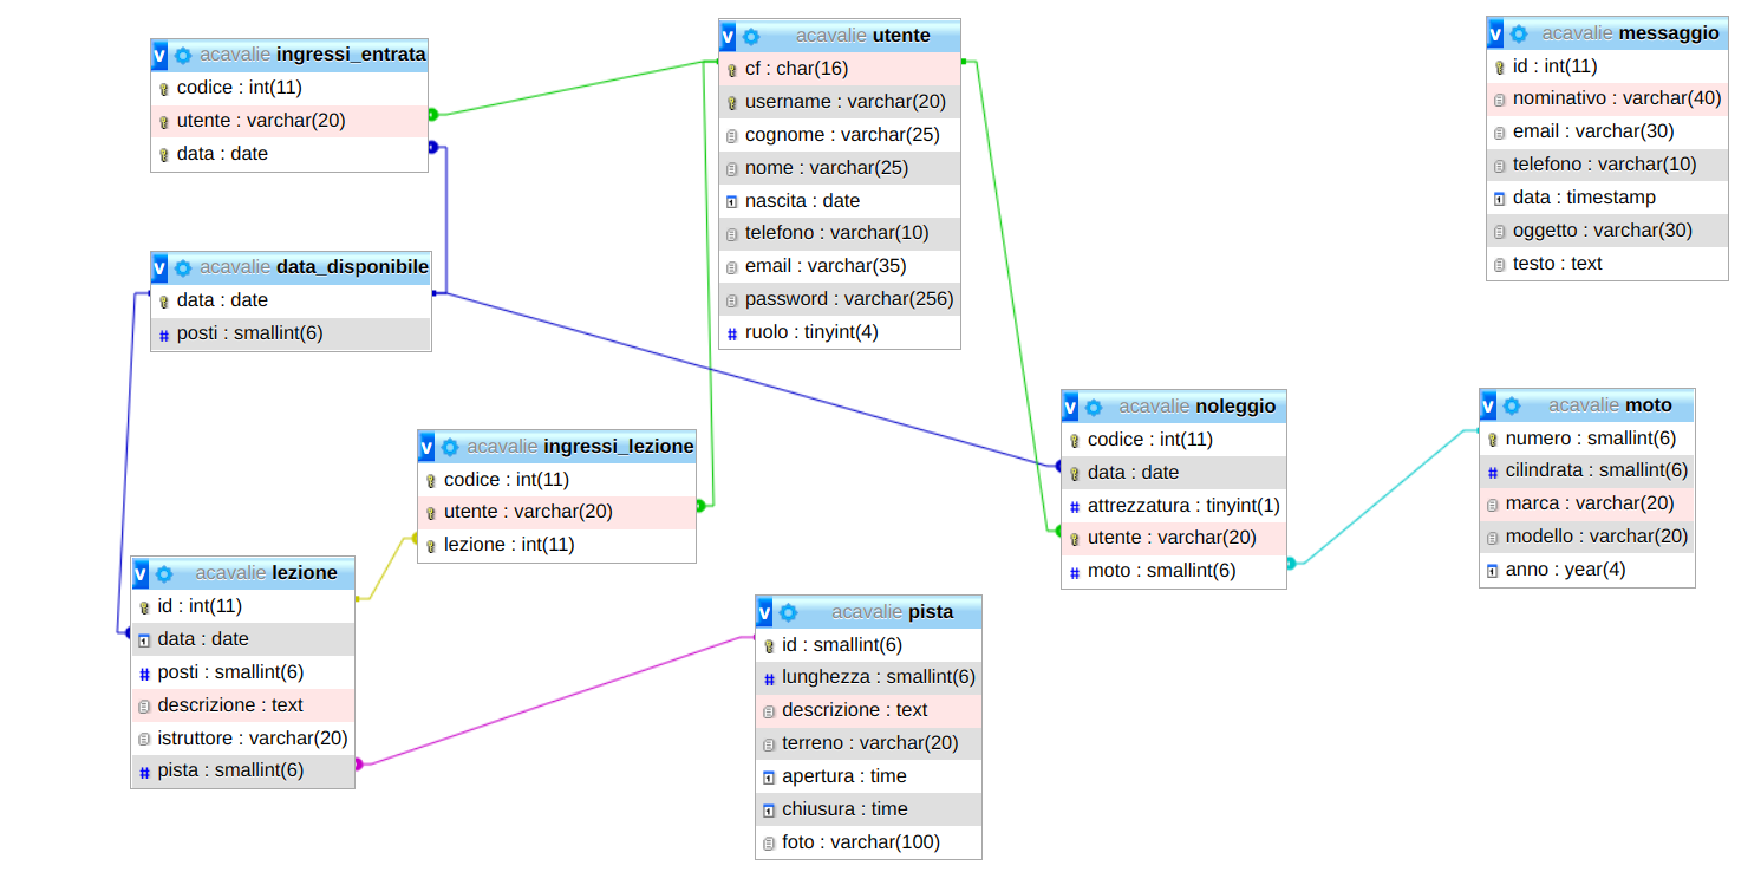
\includegraphics[scale=0.4]{./res/schemaSQL.pdf}
    \centering
    \caption{Schema SQL}
\end{figure}
